\section{Extending \texttt{Min-p's} NLP Benchmark Evaluations}
\label{sec:nlp_benchmark_evals}

We next turned to the original paper's NLP benchmark evaluations of several models on GSM8K with Chain-of-Thought \citep{cobbe2021gsm8k} and GPQA (5-shot) \citep{rein2023gpqa}, which concluded that ``\texttt{min-p} sampling achieves superior performance across benchmarks and temperatures.''

% We investigated this claim through rigorous, large-scale experiments on one of these benchmarks, GSM8K, to determine if \texttt{min-p}’s purported superiority holds under thorough hyperparameter exploration.

\subsection{Thorough Hyperparameter Sweep on GSM8K Contradicts Claim of \texttt{Min-p}'s Superiority}
\label{sec:nlp_evals:subsec:gsm8k}

\begin{figure}[t!]
    \centering
    
\includegraphics[width=0.8\linewidth]{figures/nlp_benchmark_evals/gsm8k_cot_llama/y=em_strict_x=N_hue=sampler_row=model_col=task.pdf}
    \caption{\textbf{\texttt{Min-P} Does Not Consistently Outperform Other Samplers on GSM8K When Controlling For Hyperparameter Volume.}
    In our first analysis, we measured how the maximum Exact Match (Strict) for each sampler improves as the number of hyperparameters increases. \texttt{Basic} sampling has only a temperature hyperparameter, and we therefore do not sweep it to the same degree.
    }
    \label{fig:gsm8k_em_strict}
\end{figure}

To test whether \texttt{min-p} indeed achieves superior performance, we conducted an extensive analysis on GSM8K CoT, sweeping the following models, samplers, hyperparameters and sampling seeds:
%
\begin{itemize}
    \item \textbf{9 Models:} Qwen 2.5 \citep{qwen2025qwen25technicalreport} 0.5B, 1.5B, 3B and 7B; Mistral 7Bv0.1 \citep{jiang2023mistral7b}; Llama \citep{grattafiori2024llama3herdmodels} 3.1 8B and 3.2 3B; Gemma 2 \citep{gemmateam2024gemma2improvingopen} 2B and 9B.
    \item \textbf{2 Model Stages:} Pre-trained (``Base'') and Post-Trained (``Instruct'').
    \item \textbf{4 Samplers:} \texttt{basic}, \texttt{top-p}, \texttt{top-k}, \texttt{min-p}.
    \item \textbf{31 Temperatures:} $0.0$ (``greedy'') to $3.0$ in increments of $0.1$.
    \item \textbf{6 Hyperparameters Per Sampler:} We chose $6$ hyperparameters per sampler, except for \texttt{basic} which has no hyperparameter beyond temperature. The values were taken from the original paper's text, appendix tables and released evaluation logs, then extended to $6$ values per sampler:
    \begin{itemize}
        \item \texttt{basic}: No hyperparameters other than temperature.
        \item \texttt{top-k}:  $k \in \{10, 30, 50, 100, 150, 200 \}$. The original paper tested $k \in \{10, 15, 20, 40, 50, 180\}$, which clusters four values between $10$ and $50$; we kept $10$ and $50$ and spread the remaining values more evenly up to $200$.
        \item \texttt{top-p}: $p \in \{0.99, 0.98, 0.95, 0.9, 0.8, 0.7 \}$. The original paper's four values $\{0.7, 0.8, 0.9, 0.95\}$ were retained and $0.98$ and $0.99$ were added toward the no-truncation end.
        \item \texttt{min-p}: $p \in \{0.01, 0.02, 0.05, 0.1, 0.2, 0.3 \}$. The original paper's four values $\{0.05, 0.1, 0.2, 0.3\}$ were retained and $0.01$ and $0.02$ were added, since the original paper describes small $p$ as the sensitive regime.
    \end{itemize}
    Temperatures were densified from the original paper's $\{0.7, 1.0, 1.5, 2.0, 3.0\}$ to $0.1$ spacing, and every sampler value was run at every temperature, whereas the original paper's released logs cover a ragged subset of the grid with one run per configuration.
    \item \textbf{3 Random Seeds for Sampling:} $\{0, 1, 2\}$
\end{itemize}



\begin{figure}[t!]
    \centering
    
\includegraphics[width=0.8\linewidth]{figures/nlp_benchmark_evals/gsm8k_cot_llama/y=diff_of_em_strict_x=N_hue=sampler_row=model_col=task.pdf}
    \caption{\textbf{\texttt{Min-P} Does Not Consistently Outperform Other Samplers on GSM8K When Controlling For Hyperparameter Volume.}
    In our second analysis, we measured how the difference between \texttt{min-p}'s highest score and the best non-\texttt{min-p} sampler's highest score changes as the number of swept hyperparameters increases. \texttt{Min-p} matches or underperforms other samplers.}
    \label{fig:gsm8k_diff_of_em_strict}
\end{figure}


We evaluated GSM8K CoT under two prompt formats (for reasons explained below) and, in Sec.~\ref{sec:nlp_evals:subsec:gpqa}, GPQA. The GSM8K CoT sweeps required $\sim6000$ Nvidia A100-hours and the GPQA sweep $\sim700$ Nvidia A100-hours (summed run times, one GPU per run).
% ; if community interest after this manuscript remains high, we can extend our sweep to \texttt{GPQA} \citep{rein2023gpqa}.
GSM8K contains a subset of samples with ambiguous language or incorrect labels that have since been identified and cleaned \citep{vendrow2025large} and that models may have been trained on GSM8K \citep{zhang2024careful}, but we used GSM8K nonetheless for consistency with the original paper. We similarly used EleutherAI's LM Eval Harness \citep{gao2021framework,biderman2024lessonstrenchesreproducibleevaluation}. 

To evaluate how performant each sampler is, we first averaged over the three sampling seeds and then conducted two complementary analyses:
\begin{enumerate}
    \item For each sampler, we subsampled an equal number of hyperparameters ranging from $N=1$ to $N=100$ and computed the maximum Exact Match (Strict) score achieved by the sampled subset of size $N$. We repeated this process $150$ times, averaging over the subsampled subsets' scores. This ``Best-of-N'' analysis \citep{nakano2021webgpt,stiennon2020learning,hughes2024bestofnjailbreaking,schaeffer2025largelanguagemonkeyspower} tells us the best possible performance each sampler will likely obtain as its hyperparameter space increases.
    
    \item For $N=1$ to $N=100$, we subsampled $N$ hyperparameters per sampler and computed the difference of the maximum Exact Match (Strict) score achieved by \texttt{min-p} minus the maximum score achieved by any other sampler. We repeated this process $150$ times, averaging over the subsampled subsets. This tells us by how much \texttt{min-p} outperforms all other samplers, controlling for the size of hyperparameter space of each sampler.
\end{enumerate}


\textbf{Both analyses reached consistent results: \texttt{min-p} does not outperform other samplers when equalizing the volume of hyperparameter space.}
Fig.~\ref{fig:gsm8k_em_strict} and Fig.~\ref{fig:gsm8k_diff_of_em_strict} respectively demonstrate that min-p is largely indistinguishable from other samplers.
% We also note that the experimental design in the original paper has a methodological limitation: because different samplers respond differently to temperature adjustments, comparing samplers at fixed temperature values may not provide a complete picture of their performance.
% Our analysis specifically seeks to correct for this bias by considering how the samplers perform when controlling for the volume of hyperparameter space.

After we showed these results to the authors, they informed us that we had run our experiments using the \href{https://github.com/EleutherAI/lm-evaluation-harness/blob/main/lm_eval/tasks/gsm8k/gsm8k-cot-llama.yaml}{``Llama''
formatting of GSM8K CoT prompts} as we used the command from the authors'
\href{https://github.com/menhguin/minp_paper/blob/main/%5BPUBLIC%5D_Min_P_Evals_Replication_for_GPQA_and_GSM8K_COT.ipynb}{public Colab notebook};
the authors \href{https://github.com/menhguin/minp_paper/commit/9ca63687df807b4276c527b9b47e65379c1b0bd6}{clarified} that ``Llama'' formatting should be used only for Llama models.
We then reran our experiments using \href{https://github.com/EleutherAI/lm-evaluation-harness/blob/main/lm_eval/tasks/gsm8k/gsm8k-cot.yaml}{standard formatting of GSM8K CoT prompts}.
The results were nearly identical (Appendix \ref{app:sec:gsm_cot_scores}), with one small difference: \texttt{min-p} does produce higher scores for 2 of 12 language models.
Again, we conclude \textbf{\texttt{min-p} does not outperform other samplers on either formatting of GSM8K CoT when controlling for hyperparameter volume}.

\subsection{Thorough Hyperparameter Sweep on GPQA Reaches the Same Conclusion}
\label{sec:nlp_evals:subsec:gpqa}

\begin{figure}[t!]
    \centering
    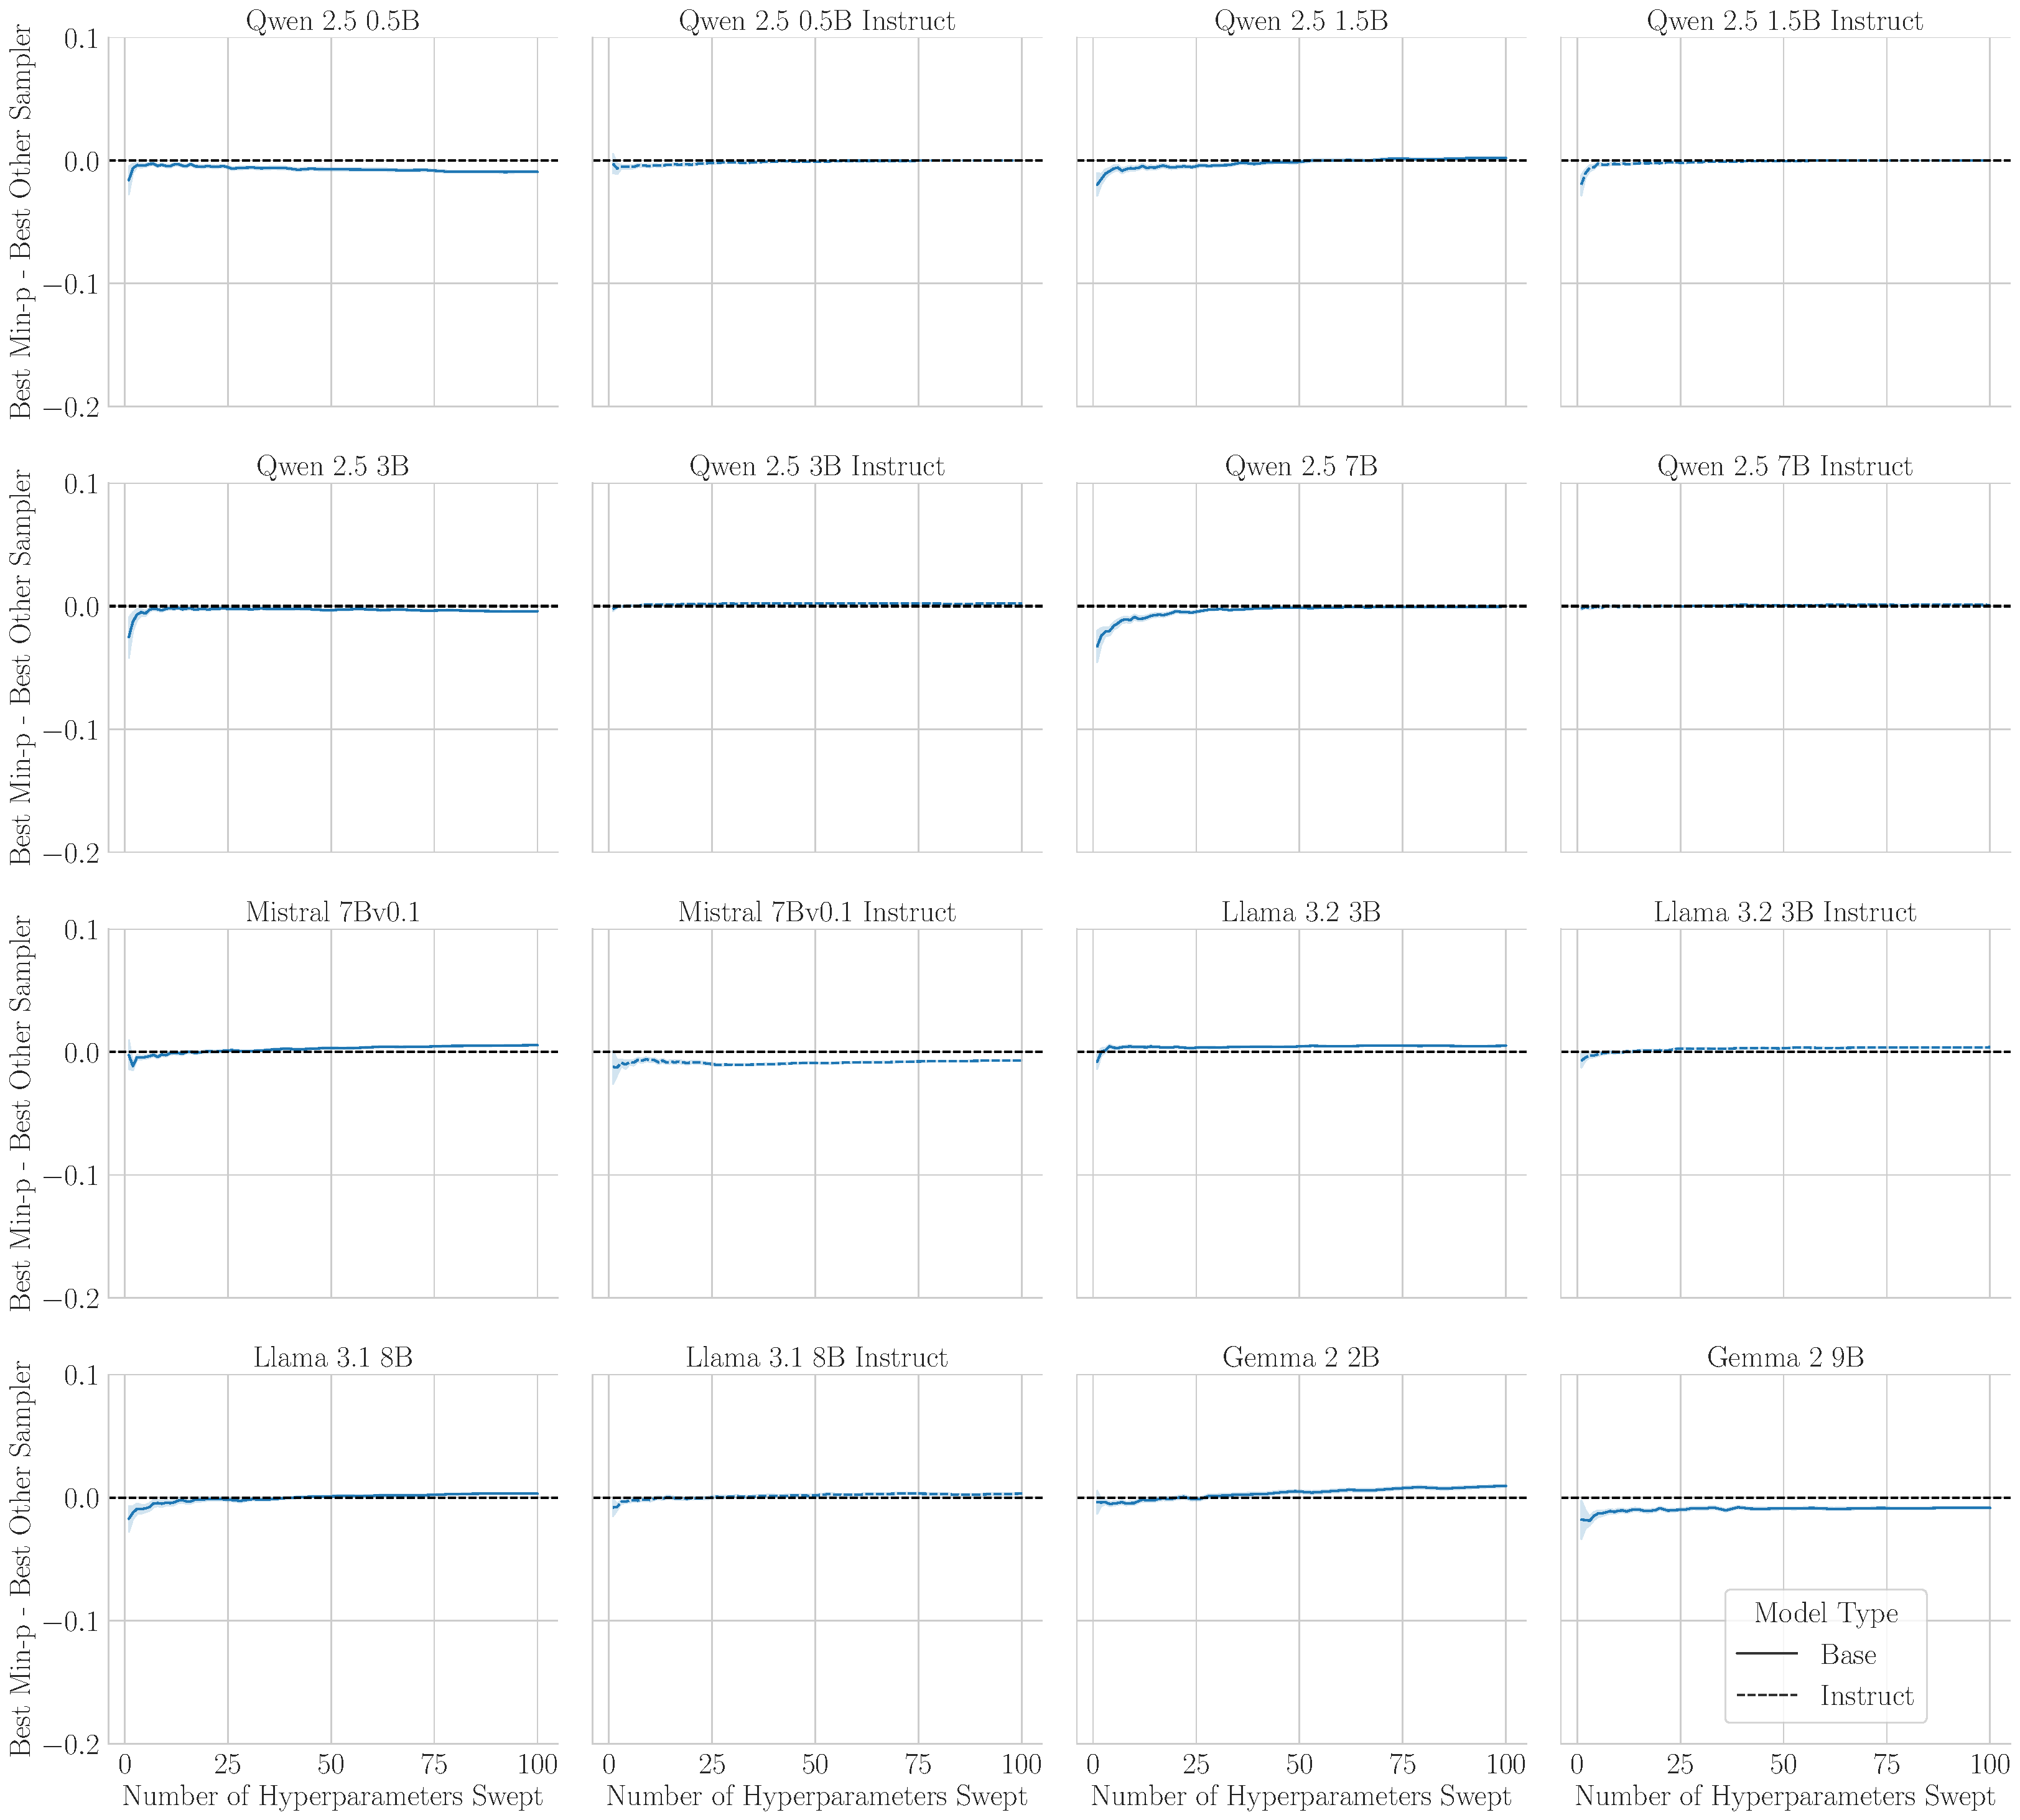
\includegraphics[width=0.8\linewidth]{figures/nlp_benchmark_evals/gpqa/y=diff_of_em_flexible_x=N_hue=sampler_row=model_col=task.pdf}
    \caption{\textbf{\texttt{Min-P} Does Not Consistently Outperform Other Samplers on GPQA When Controlling For Hyperparameter Volume.} Difference between the best-of-$N$ score of \texttt{min-p} and the best-of-$N$ score of the best other sampler on GPQA (5-shot, flexible-extract exact match), using the same models, samplers, temperatures, sampler values and seeds as the GSM8K CoT sweep. For all 16 models the difference stays within $1.3$ percentage points (six of GPQA's 448 questions) at every $N$: at the full sweep, \texttt{min-p}'s best configuration is numerically higher on 9 models, equal on 3 and lower on 4, and every margin is smaller than the seed-to-seed standard deviation of a single configuration ($\approx 1.5$ points). Gemma 2 2B Instruct and Gemma 2 9B Instruct are omitted because their GPQA runs produced no scores under the pinned \texttt{lm-eval} version. Best-of-$N$ scores per sampler are shown in Appendix~\ref{app:sec:gpqa_scores}.}
    \label{fig:gpqa_diff_of_em}
\end{figure}

The original paper also evaluated GPQA \citep{rein2023gpqa}, and its claim of superiority was stated ``across benchmarks.''
We therefore repeated the sweep of Sec.~\ref{sec:nlp_evals:subsec:gsm8k} on GPQA (5-shot) with the identical grid of models, samplers, temperatures, sampler values and seeds, and applied the same two best-of-$N$ analyses.
Two Gemma 2 Instruct models produced no GPQA scores under the pinned \texttt{lm-eval} version and are omitted, leaving 16 models.
The results (Fig.~\ref{fig:gpqa_diff_of_em}; Appendix~\ref{app:sec:gpqa_scores}) match those on GSM8K CoT: once every sampler is given the same number of hyperparameter configurations, the best \texttt{min-p} configuration is within $1.3$ percentage points of the best other sampler on every model, numerically higher on 9, equal on 3 and lower on 4, with every margin smaller than the seed-to-seed noise of a single configuration.
\textbf{On both of the original paper's NLP benchmarks, \texttt{min-p} does not outperform other samplers when controlling for hyperparameter volume.}
